\section{Schelling Segregation Model}\label{ch:app2}

Schelling's original work sought to answer questions regarding how segregation could arise in an environment like his, which was the USA in the 1960s, where segregation occurred for a long time even after the civil rights movement tried to contrast it \cite{sowell_knowledge_1996}. Segregation doesn't happen only in static environments tough, indeed it can emerge in more dynamic situations, where for instance migration and assimilation play a role in shaping communities \cite{sowell_social_2023}. \\
Plot \ref{plt:migration} displays the results of adding a migration dynamic to Schelling's 1D model described in chapter \ref{ch:2}. In particular, two probabilities were defined, named enter and leave. The first one determines the probability that at the end of each cycle agents of majority type will emigrate, while the second one determines the probability vacancies will be filled with agents of minority types. \\ 
\begin{figure}[htbp]
    \centering
    \begin{minipage}[t]{0.48\linewidth}
        \centering
        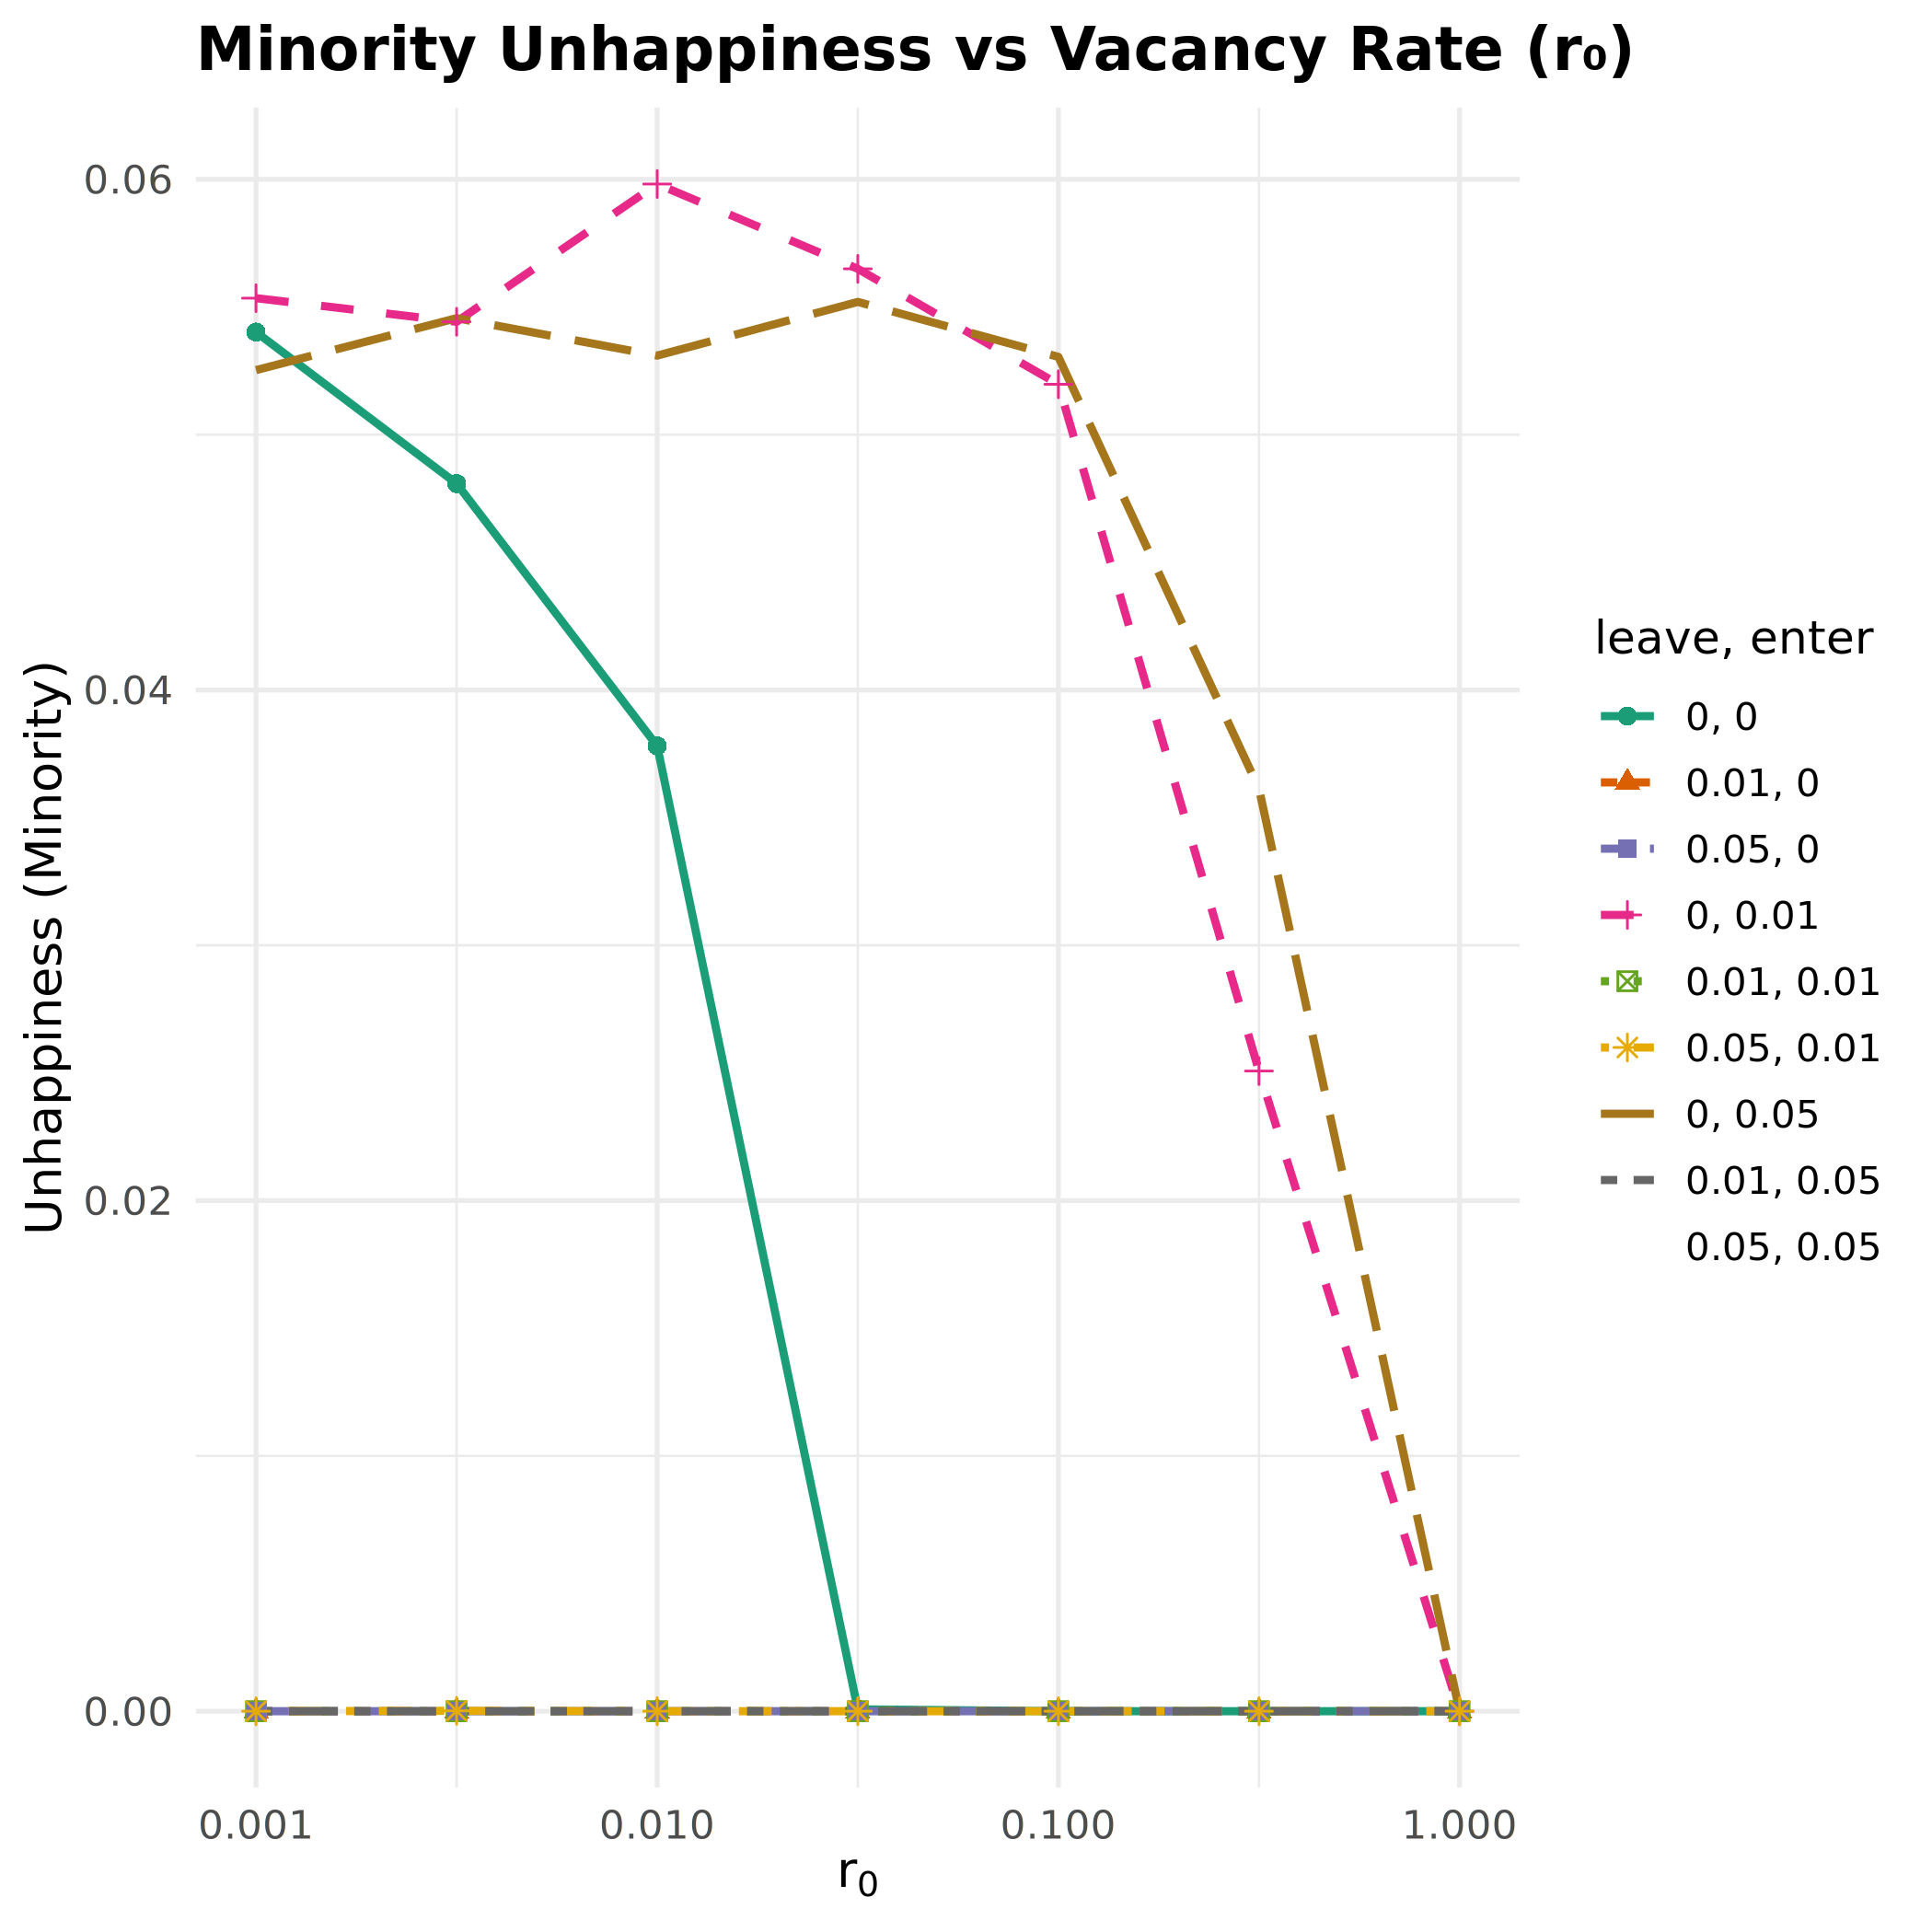
\includegraphics[width=\linewidth]{images/segregation_plot_migration_minority_.png}
        \caption{Unhappiness of agents of the minority type.}
        \label{fig:immigration}
    \end{minipage}
    \hfill
    \begin{minipage}[t]{0.48\linewidth}
        \centering
        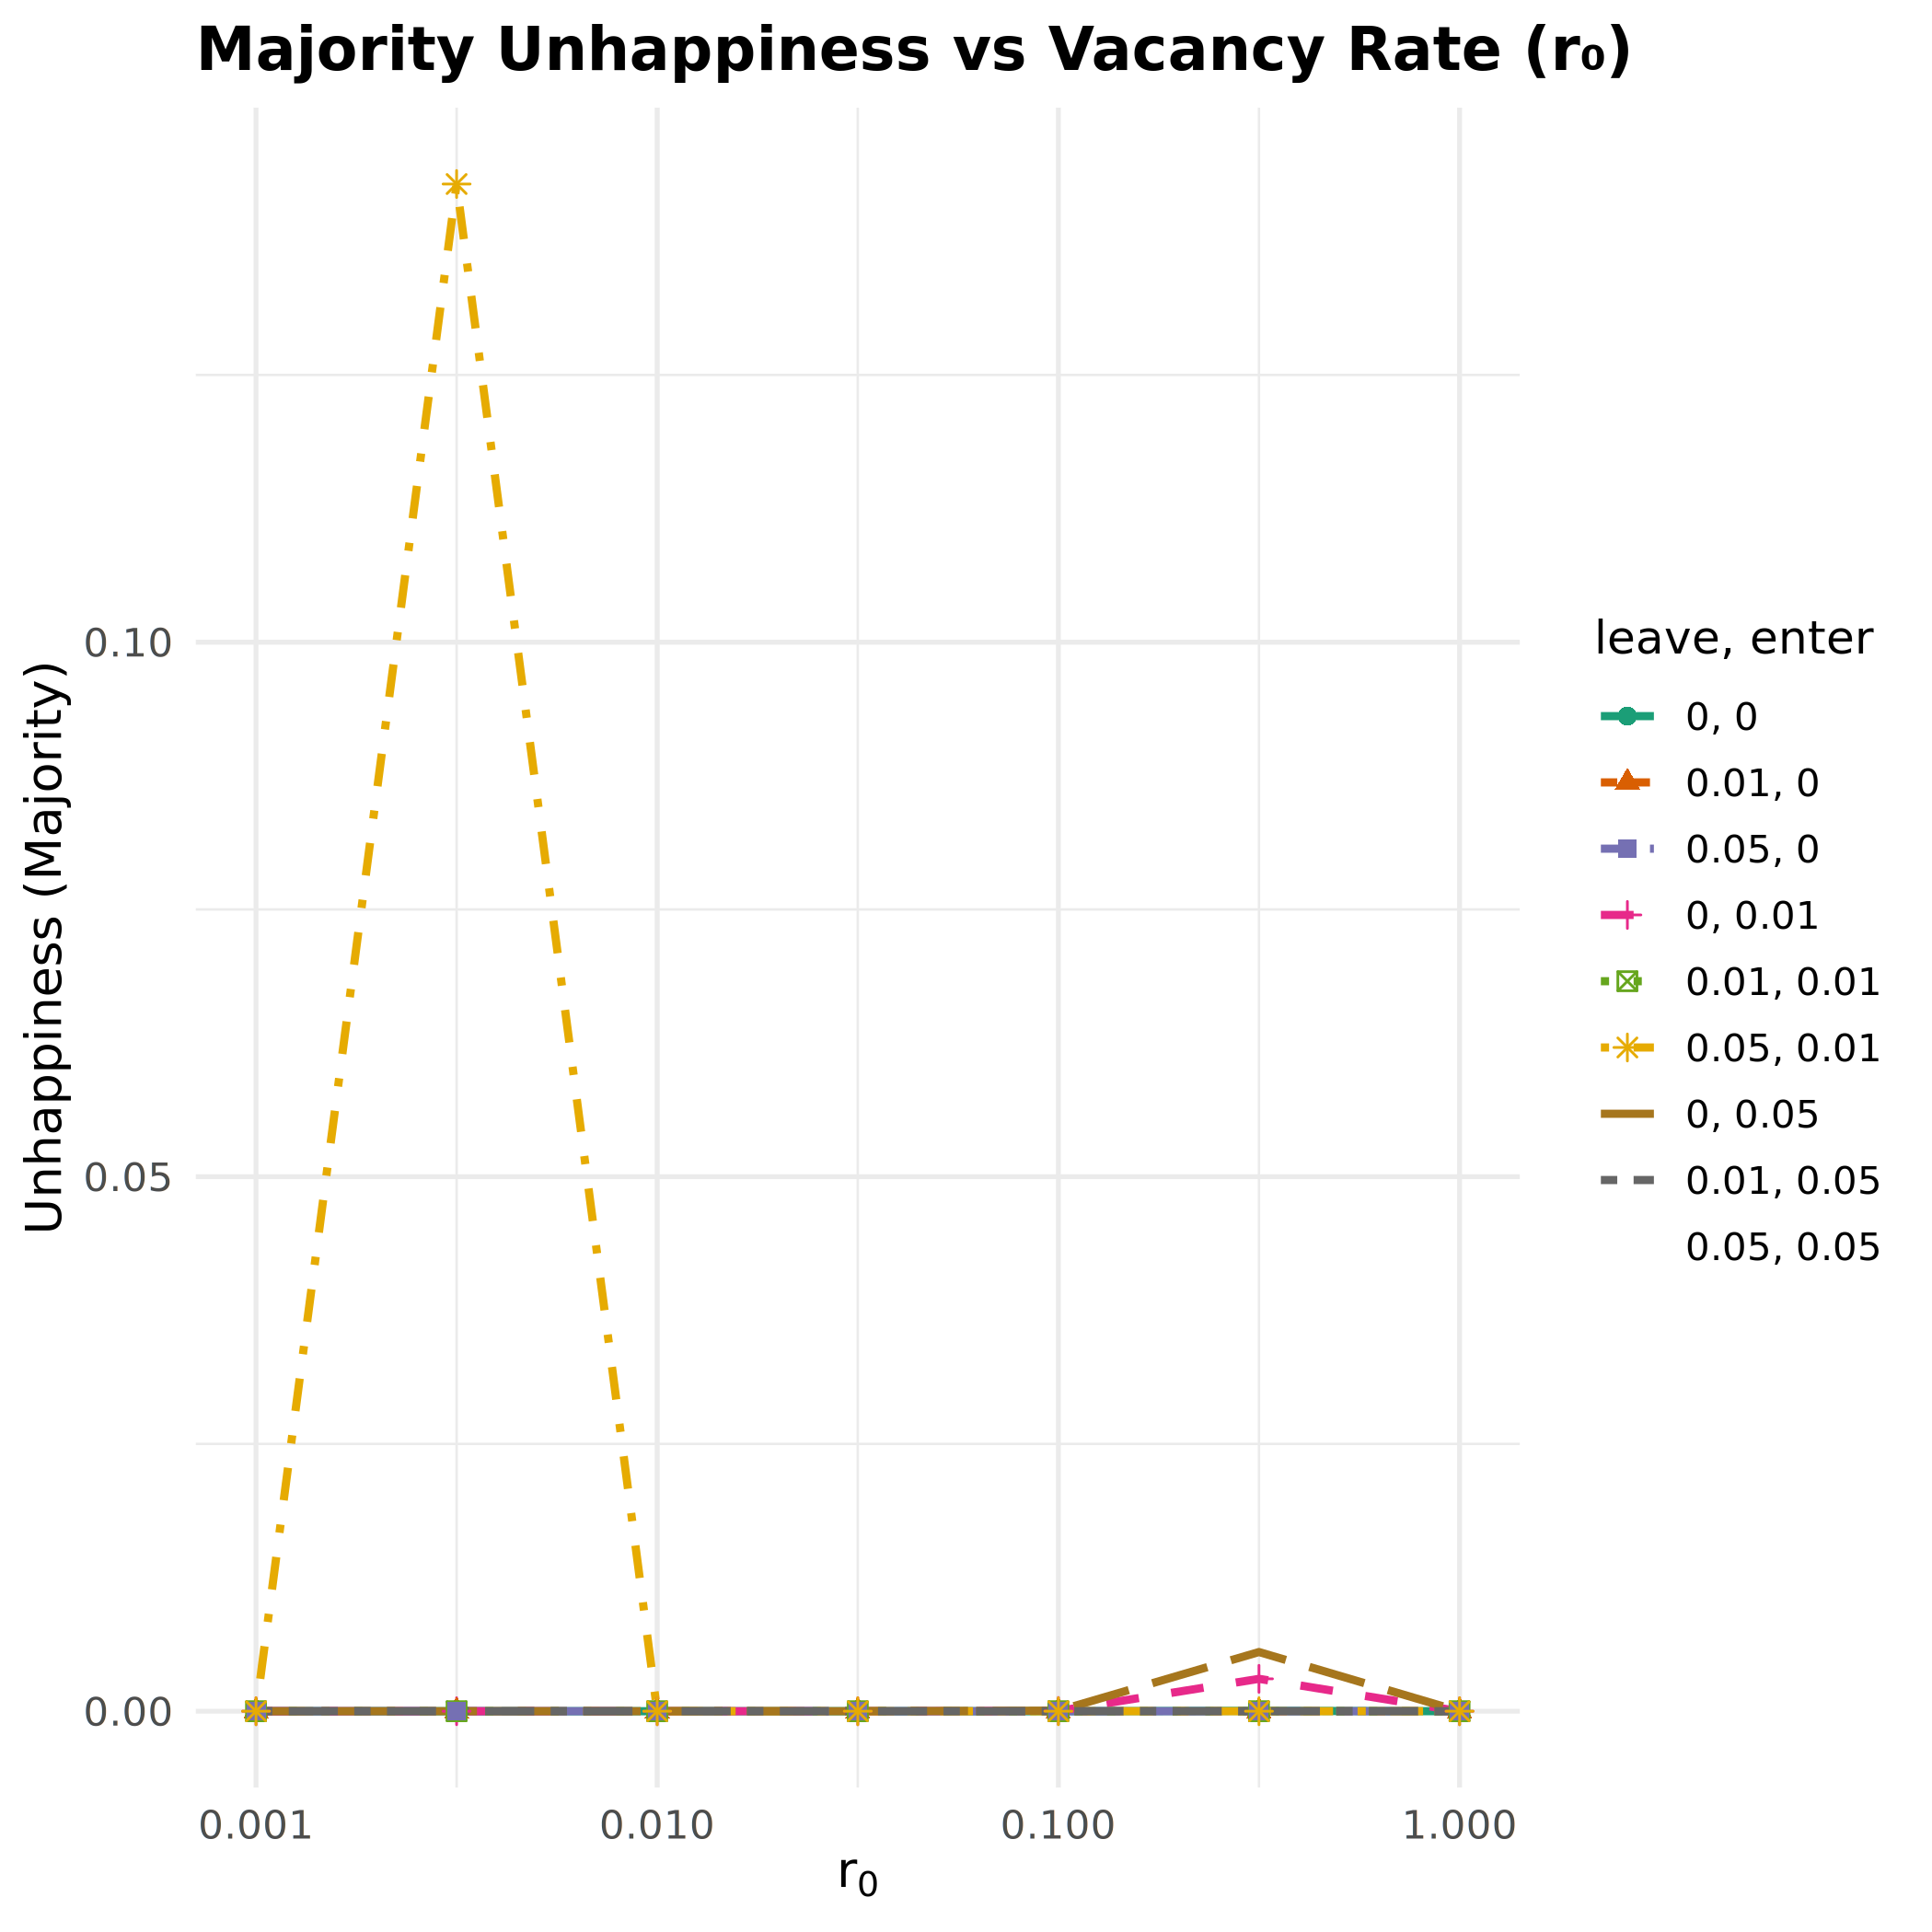
\includegraphics[width=\linewidth]{images/segregation_plot_migration_majority_.png}
        \caption{Unhappiness of agents of the majority type.}
        \label{fig:emigration}
    \end{minipage}
    \caption{}
    \label{plt:migration}
\end{figure}

Due to limits of computational resources, the plots have been done for only a few values of $r_0$ (seven actually), few replications (again, seven) and few iteration steps. Nevertheless, it's interesting to note that it does seem the case that high immigration rate will reduce the unhappiness of agents of minority type, though it might increase the unhappiness of the agents of originally majority type, especially if paired with high emigration rates on their part. \\

Another overlooked aspect of segregation is how agents interacting with each other might become more alike, as shown in Axelrod's model of social influence \cite{axelrod_dissemination_1997}. Since incorporating both models could be too complicated for the scope of this project, what will be presented here is a simpler implementation, where on top of the dynamics of the basic 1D Schelling model, at each iteration an unhappy agent, with a certain probability, might become of the same type as the agents surrounding him. The result of such dynamics is shown in plot \ref{fig:assimilation}, where the average of 20 replications of the dynamics (with few iterations only within each replication though) shows that adding an assimilation rate lowers unhappiness. The implications of this suggest that cultures that are already similar and compatible, and thus more likely to assimilate each other, might not give rise to significant segregation.
\begin{table}[ht]
\centering
% latex table generated in R 4.4.1 by xtable 1.8-4 package
% Sun Jul 13 17:45:38 2025
\begin{table}[ht]
\centering
\begin{tabular}{|ccc}
  \hline
r0 & p_assim & u_min \\ 
  \hline
0.00 & 0.00 & 0.30 \\ 
  0.00 & 0.00 & 0.31 \\ 
  0.00 & 0.00 & 0.31 \\ 
  0.00 & 0.00 & 0.30 \\ 
  0.00 & 0.00 & 0.31 \\ 
  0.01 & 0.00 & 0.30 \\ 
  0.01 & 0.00 & 0.30 \\ 
  0.01 & 0.00 & 0.30 \\ 
  0.02 & 0.00 & 0.30 \\ 
  0.03 & 0.00 & 0.30 \\ 
  0.04 & 0.00 & 0.30 \\ 
  0.05 & 0.00 & 0.31 \\ 
  0.08 & 0.00 & 0.31 \\ 
  0.11 & 0.00 & 0.33 \\ 
  0.16 & 0.00 & 0.33 \\ 
  0.23 & 0.00 & 0.34 \\ 
  0.34 & 0.00 & 0.33 \\ 
  0.48 & 0.00 & 0.27 \\ 
  0.70 & 0.00 & 0.03 \\ 
  1.00 & 0.00 & 0.00 \\ 
  0.00 & 0.00 & 0.29 \\ 
  0.00 & 0.00 & 0.29 \\ 
  0.00 & 0.00 & 0.28 \\ 
  0.00 & 0.00 & 0.28 \\ 
  0.00 & 0.00 & 0.28 \\ 
  0.01 & 0.00 & 0.29 \\ 
  0.01 & 0.00 & 0.29 \\ 
  0.01 & 0.00 & 0.29 \\ 
  0.02 & 0.00 & 0.29 \\ 
  0.03 & 0.00 & 0.29 \\ 
  0.04 & 0.00 & 0.29 \\ 
  0.05 & 0.00 & 0.29 \\ 
  0.08 & 0.00 & 0.30 \\ 
  0.11 & 0.00 & 0.31 \\ 
  0.16 & 0.00 & 0.32 \\ 
  0.23 & 0.00 & 0.33 \\ 
  0.34 & 0.00 & 0.32 \\ 
  0.48 & 0.00 & 0.25 \\ 
  0.70 & 0.00 & 0.03 \\ 
  1.00 & 0.00 & 0.00 \\ 
  0.00 & 0.00 & 0.19 \\ 
  0.00 & 0.00 & 0.19 \\ 
  0.00 & 0.00 & 0.19 \\ 
  0.00 & 0.00 & 0.19 \\ 
  0.00 & 0.00 & 0.19 \\ 
  0.01 & 0.00 & 0.20 \\ 
  0.01 & 0.00 & 0.19 \\ 
  0.01 & 0.00 & 0.20 \\ 
  0.02 & 0.00 & 0.19 \\ 
  0.03 & 0.00 & 0.19 \\ 
  0.04 & 0.00 & 0.20 \\ 
  0.05 & 0.00 & 0.20 \\ 
  0.08 & 0.00 & 0.21 \\ 
  0.11 & 0.00 & 0.21 \\ 
  0.16 & 0.00 & 0.22 \\ 
  0.23 & 0.00 & 0.21 \\ 
  0.34 & 0.00 & 0.21 \\ 
  0.48 & 0.00 & 0.16 \\ 
  0.70 & 0.00 & 0.00 \\ 
  1.00 & 0.00 & 0.00 \\ 
  0.00 & 0.00 & 0.13 \\ 
  0.00 & 0.00 & 0.13 \\ 
  0.00 & 0.00 & 0.13 \\ 
  0.00 & 0.00 & 0.13 \\ 
  0.00 & 0.00 & 0.13 \\ 
  0.01 & 0.00 & 0.13 \\ 
  0.01 & 0.00 & 0.13 \\ 
  0.01 & 0.00 & 0.13 \\ 
  0.02 & 0.00 & 0.13 \\ 
  0.03 & 0.00 & 0.13 \\ 
  0.04 & 0.00 & 0.13 \\ 
  0.05 & 0.00 & 0.13 \\ 
  0.08 & 0.00 & 0.14 \\ 
  0.11 & 0.00 & 0.14 \\ 
  0.16 & 0.00 & 0.14 \\ 
  0.23 & 0.00 & 0.14 \\ 
  0.34 & 0.00 & 0.13 \\ 
  0.48 & 0.00 & 0.09 \\ 
  0.70 & 0.00 & 0.00 \\ 
  1.00 & 0.00 & 0.00 \\ 
  0.00 & 0.01 & 0.00 \\ 
  0.00 & 0.01 & 0.00 \\ 
  0.00 & 0.01 & 0.00 \\ 
  0.00 & 0.01 & 0.00 \\ 
  0.00 & 0.01 & 0.00 \\ 
  0.01 & 0.01 & 0.00 \\ 
  0.01 & 0.01 & 0.00 \\ 
  0.01 & 0.01 & 0.00 \\ 
  0.02 & 0.01 & 0.00 \\ 
  0.03 & 0.01 & 0.00 \\ 
  0.04 & 0.01 & 0.00 \\ 
  0.05 & 0.01 & 0.00 \\ 
  0.08 & 0.01 & 0.00 \\ 
  0.11 & 0.01 & 0.00 \\ 
  0.16 & 0.01 & 0.00 \\ 
  0.23 & 0.01 & 0.00 \\ 
  0.34 & 0.01 & 0.00 \\ 
  0.48 & 0.01 & 0.00 \\ 
  0.70 & 0.01 & 0.00 \\ 
  1.00 & 0.01 & 0.00 \\ 
   \hline
\end{tabular}
\caption{Table generated from assimilation.csv} 
\end{table}
\end{table}


At this point, it could be interesting combining both concepts, in order to get a realistic intuition of how immigration might lead to segregation. An attempt to do this is presented in figure \ref{fig:last}, where one can see the average unhappiness across seven replications of several combinations of both assimilation and migration dynamics. Again, high immigration with little-to-no assimilation causes the majority to be surprisingly unhappy, whereas a more balanced net-migration and a good assimilation rate allow both minority and majority agents to have low unhappiness.
\begin{figure}[htbp]
    \centering
    \begin{minipage}[t]{0.48\linewidth}
        \centering
        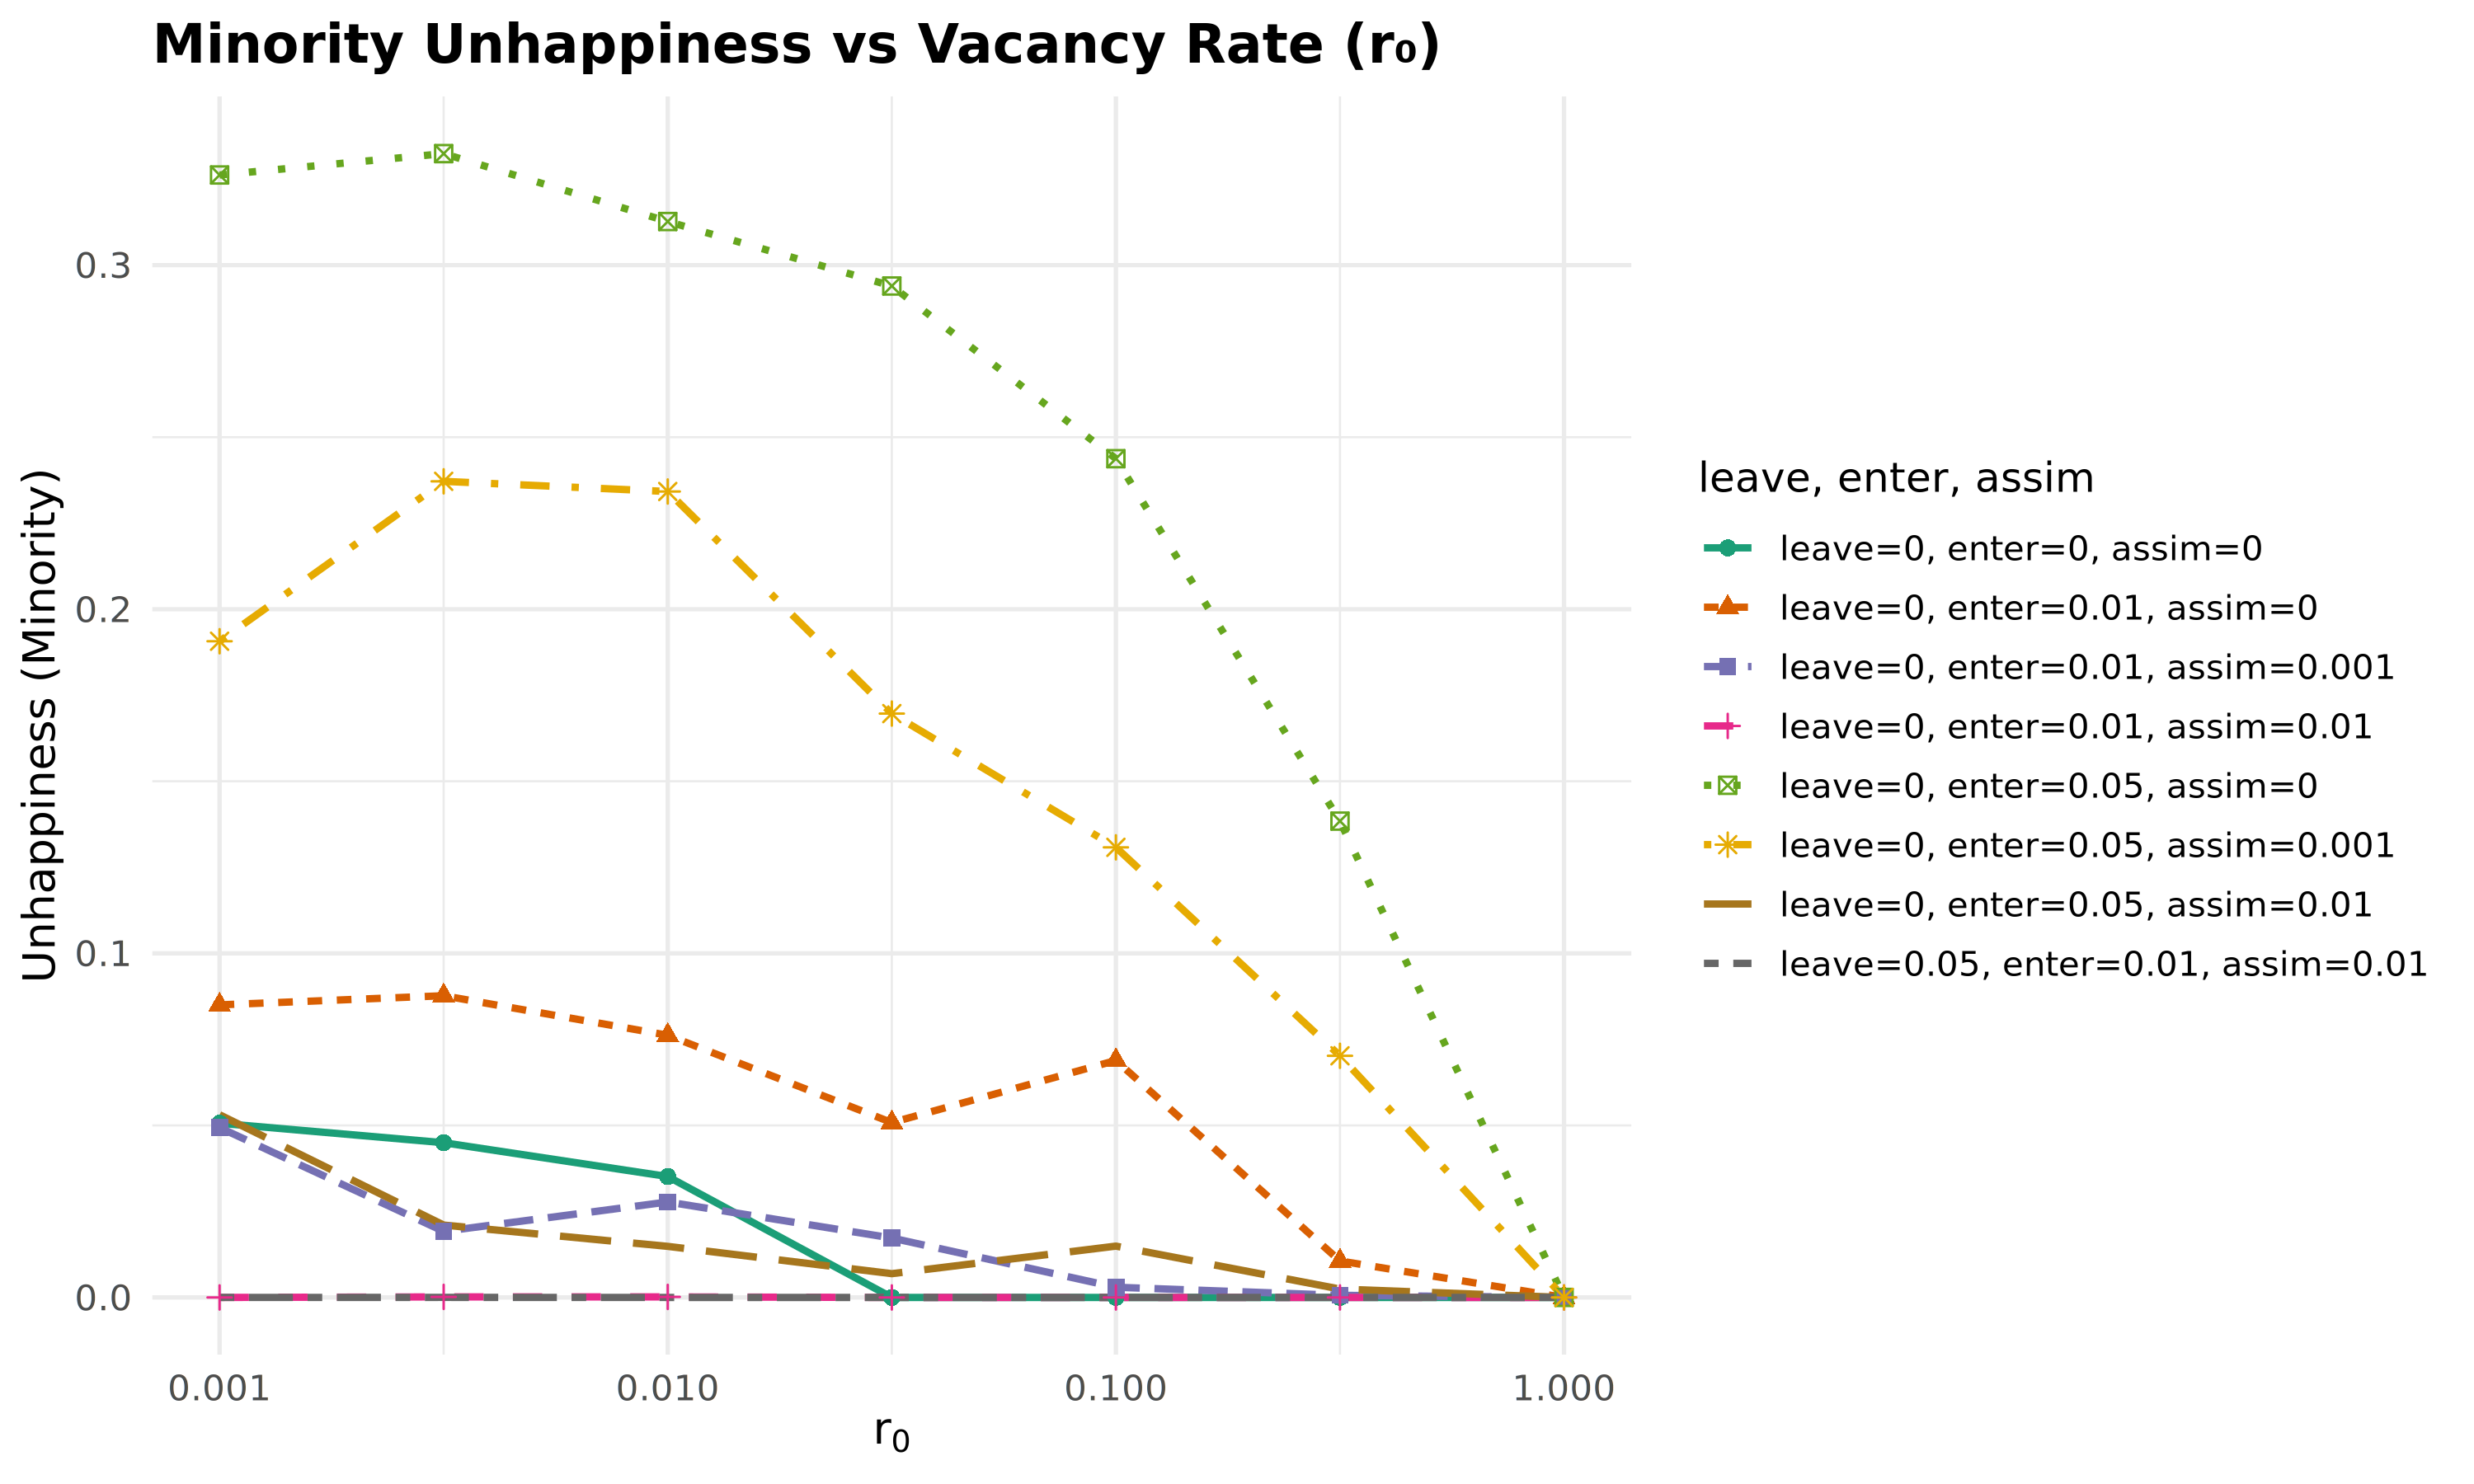
\includegraphics[width=\linewidth]{images/segregation_plot_migration_ass_minority_fixed.png}
        \caption{}
        
    \end{minipage}
    \hfill
    \begin{minipage}[t]{0.48\linewidth}
        \centering
        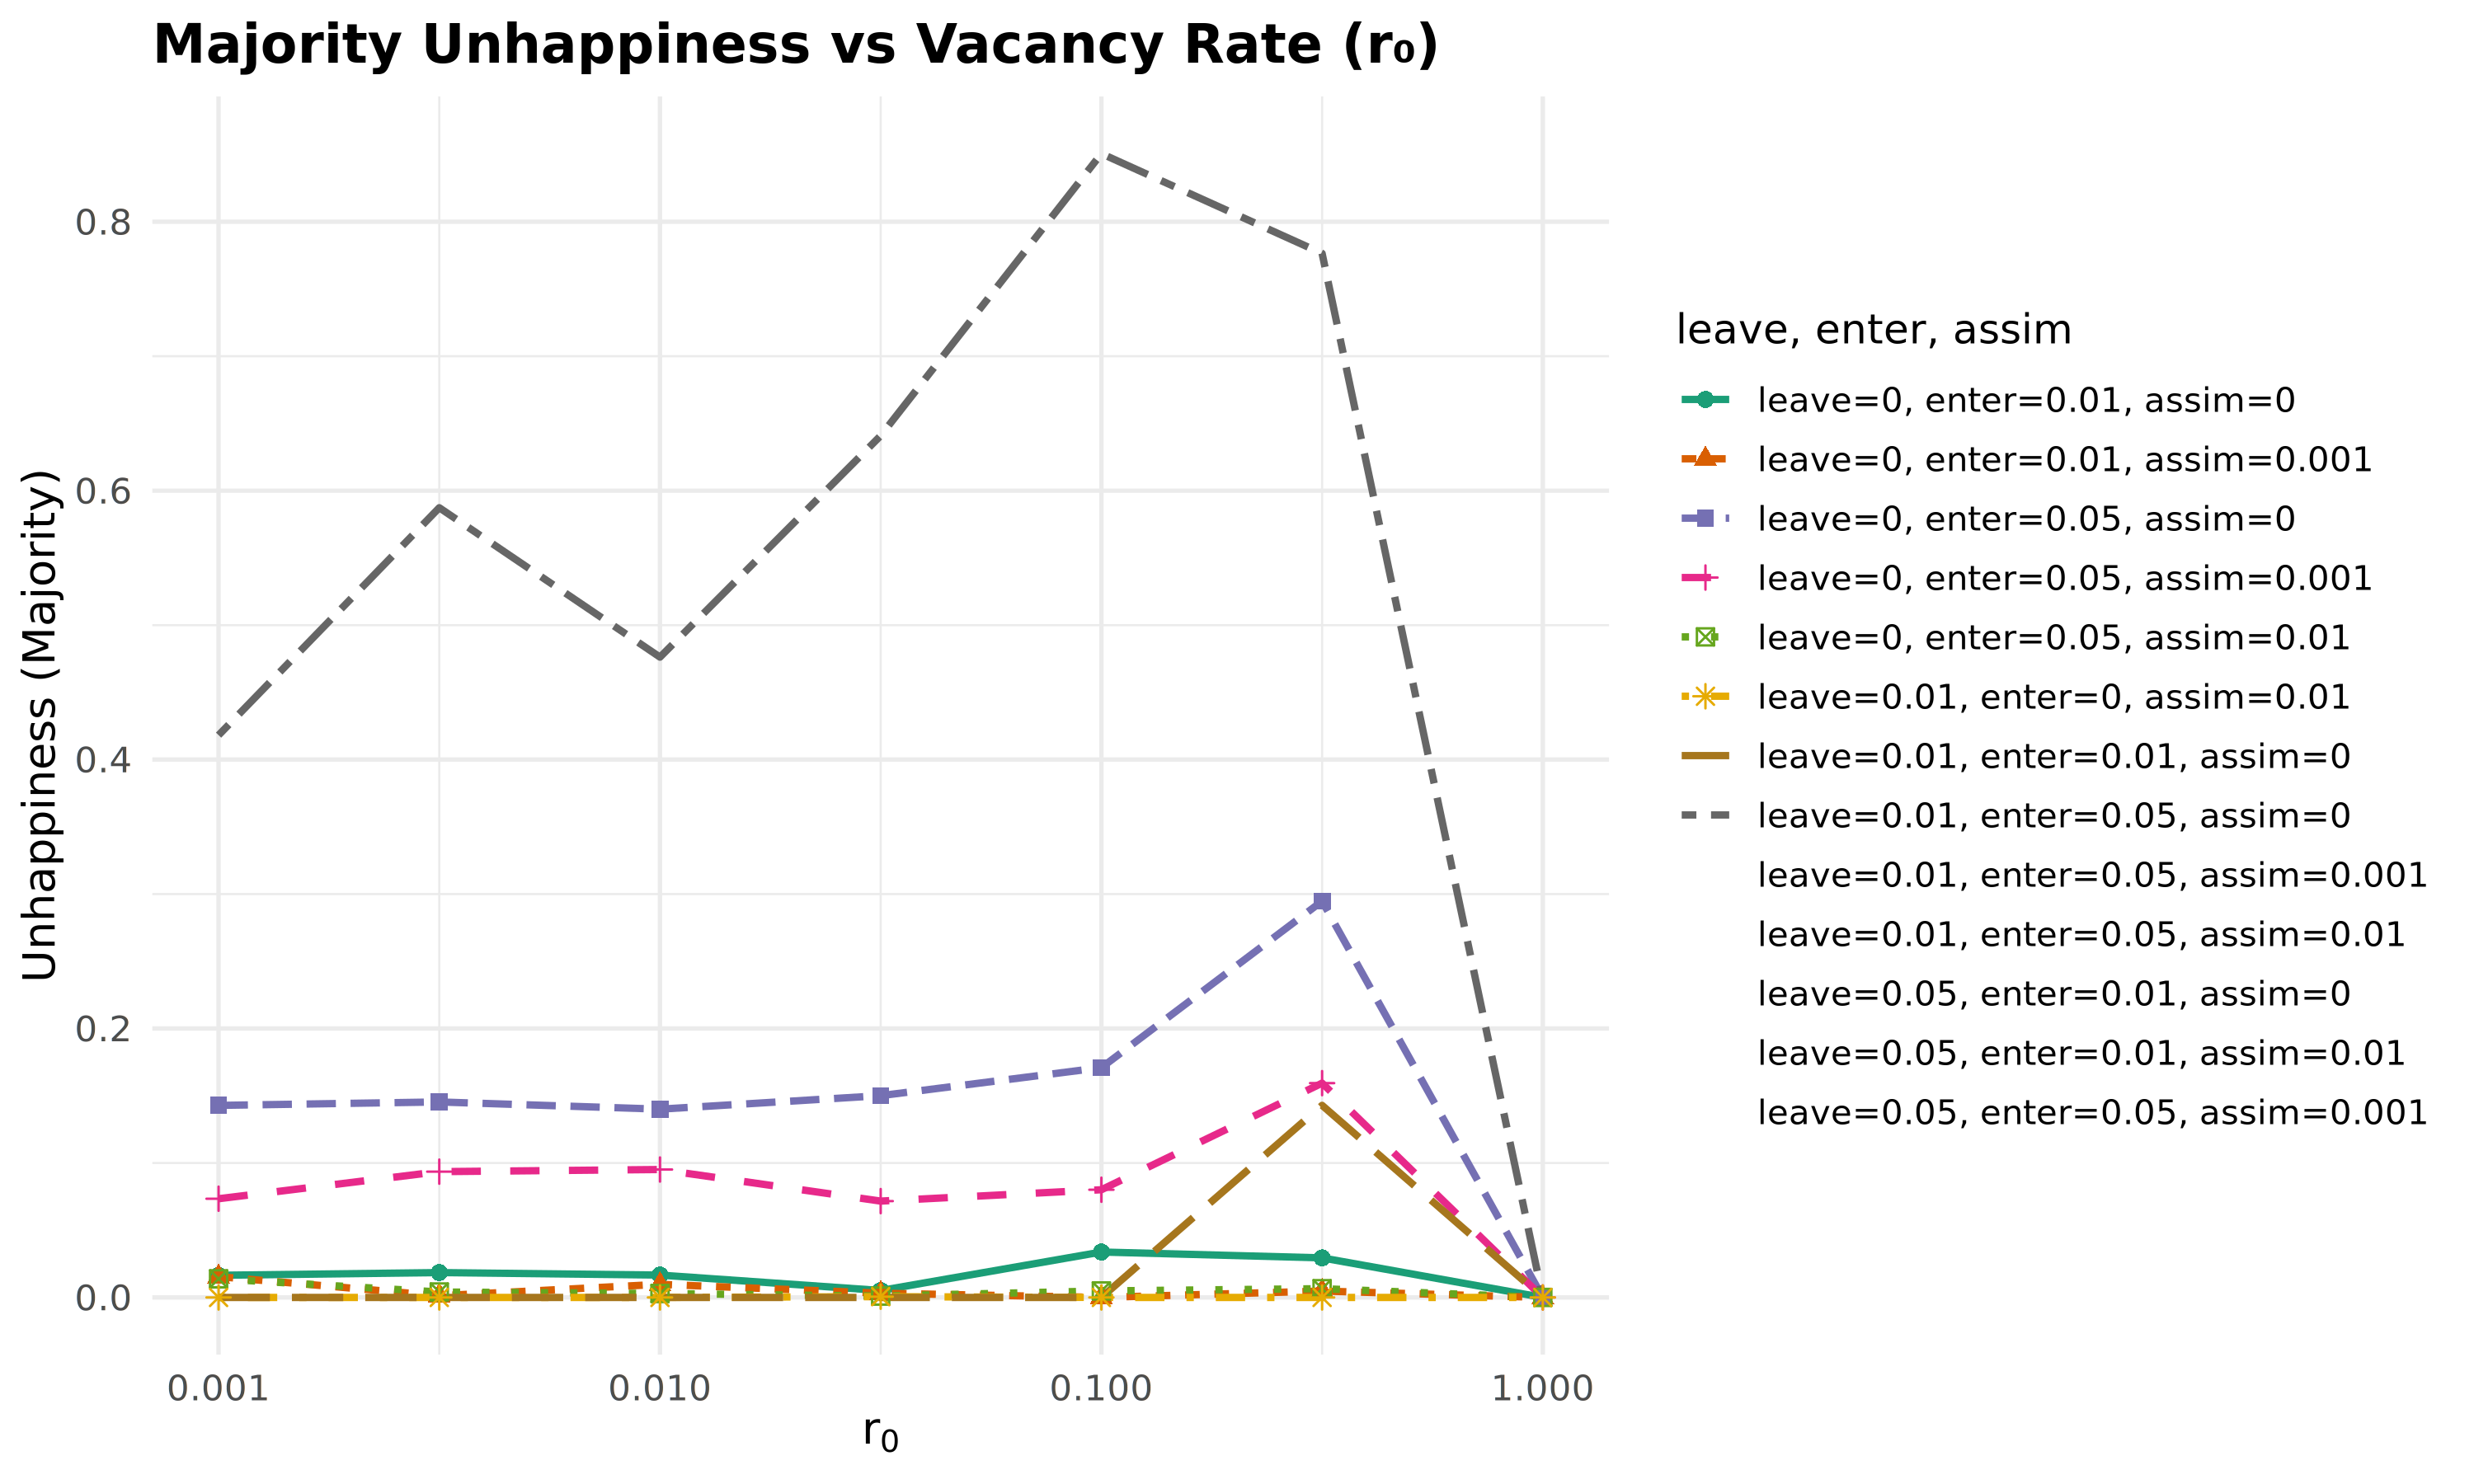
\includegraphics[width=\linewidth]{images/segregation_plot_migration_ass_majority_fixed.png}
        \caption{}
        
    \end{minipage}
    \caption{Segregation with both migration and assimilation dynamics. Only most relevant combinations have been plotted.}
    \label{fig:last}
    
\end{figure}
